\section{Flows and Cuts} 

\subsection{Max-Flow Min-Cut Theorem} 

  \begin{definition}[Flow Network]
    Given a nonnegative weighted directed graph $G(V, E)$, we can define the weights to be the \textbf{capacity} $C: E \rightarrow \mathbb{R}^+$ of some commodity that can travel through the edge. Say that we have a source node $s \in V$ and a sink/destination node $t \in V$. This is called a \textbf{flow network}.
  \end{definition}

  \begin{definition}[Flow]
    Given a flow network, a \textbf{flow} is a function $f: E \rightarrow \mathbb{R}^+$ satisfying 
    \begin{enumerate}
      \item \textit{Conservation}. What flows in must always flow out. For all $v \neq s, t$, we have 
        \begin{equation}
          \sum_{(u \rightarrow v) \in E} f(u \rightarrow v) = \sum_{(v \rightarrow w) \in E} f(v \rightarrow w)
        \end{equation}

      \item \textit{Feasibility}. We cannot exceed the capacity. For all $e \in E$, 
        \begin{equation}
          0 \leq f(e) \leq C(e)
        \end{equation}
    \end{enumerate}
    The \textbf{value} of a flow represents the actual/realized amount of the commodity that we can push through the graph
    \begin{equation}
      |f| = \sum_{(s \rightarrow u) \in E}  f(s \rightarrow u) - \sum_{(u \rightarrow s) \in E}  f(u \rightarrow s) 
    \end{equation} 
    where we need to subtract the right expression to avoid loops. 
  \end{definition}

  \begin{figure}[H]
    \centering
    \begin{tikzpicture}[
        node distance=2.5cm,
        vertex/.style={circle, draw, minimum size=0.8cm},
        auto,
        >=Stealth
    ]

    % Nodes with increased horizontal spacing
    \node[vertex] (s) at (0,0) {s};
    \node[vertex] (a) at (3,2) {};
    \node[vertex] (b) at (6,2) {};
    \node[vertex] (c) at (3,-2) {};
    \node[vertex] (d) at (6,-2) {};
    \node[vertex] (t) at (9,0) {t};

    % Edges with colored fraction labels
    \draw[->] (s) -- node[above] {$\frac{\color{red}10}{\color{blue}20}$} (a);
    \draw[->] (s) -- node[below] {$\frac{\color{red}0}{\color{blue}10}$} (c);
    \draw[->] (a) -- node[above] {$\frac{\color{red}0}{\color{blue}5}$} (b);
    \draw[->] (a) -- node[below] {$\frac{\color{red}10}{\color{blue}10}$} (c);
    \draw[->] (b) -- node[above] {$\frac{\color{red}5}{\color{blue}15}$} (t);
    \draw[->] (b) -- node[right] {$\frac{\color{red}5}{\color{blue}20}$} (d);
    \draw[->] (c) -- node[below] {$\frac{\color{red}10}{\color{blue}10}$} (d);
    \draw[->] (d) -- node[below] {$\frac{\color{red}5}{\color{blue}20}$} (t);
    \draw[<-] (c) -- node[above] {$\frac{\color{red}0}{\color{blue}15}$} (b);

    \end{tikzpicture}
    \caption{The red values represent the flow. The blue values represent the capacity. The value of the above flow is 10.} 
    \label{fig:flow}
  \end{figure}

  Now let's revisit cuts. 

  \begin{definition}[Cuts]
    Given a flow network, a s-t \textbf{cut} is a partition of $V = S \sqcup T$ s.t. $s \in S, t \in T$. The \textbf{value}, or \textbf{capacity}, of a cut is defined as the capacity of its edges 
    \begin{equation}
      ||S, T|| = \sum_{u in S} \sum_{v \in T} C(u \rightarrow v)
    \end{equation}
  \end{definition}

  \begin{figure}[H]
    \centering 
    \begin{tikzpicture}[
        node distance=2.5cm,
        vertex/.style={circle, draw, minimum size=0.8cm},
        auto,
        >=Stealth
    ]

    % Nodes with increased horizontal spacing
    \node[vertex] (s) at (0,0) {s};
    \node[vertex] (a) at (3,2) {};
    \node[vertex] (b) at (6,2) {};
    \node[vertex] (c) at (3,-2) {};
    \node[vertex] (d) at (6,-2) {};
    \node[vertex] (t) at (9,0) {t};

    % Edges with upright colored fraction labels
    \draw[->] (s) -- node[above] {$\color{blue}20$} (a);
    \draw[->] (s) -- node[below] {$\color{blue}10$} (c);
    \draw[->] (a) -- node[above] {$\color{blue}5$} (b);
    \draw[->] (a) -- node[left] {$\color{blue}10$} (c);
    \draw[->] (b) -- node[above] {$\color{blue}15$} (t);
    \draw[->] (b) -- node[right] {$\color{blue}20$} (d);
    \draw[->] (c) -- node[below] {$\color{blue}10$} (d);
    \draw[->] (d) -- node[below] {$\color{blue}20$} (t);
    \draw[<-] (c) -- node[right] {$\color{blue}15$} (b);

    % Draw the cut (add this on background layer to appear behind nodes)
    \begin{scope}[on background layer]
        \draw[dashed, thick, gray] (4.5,-3) -- (4.5,3);
        
        % Add labels for the sets
        \node at (2,2.5) {S};
        \node at (7,2.5) {T};
    \end{scope}

    \end{tikzpicture}
    \caption{This cut has capacity 15. Note that the cut going from right to left is not included since this is a S-T cut. } 
    \label{fig:cut}
  \end{figure}

  We now introduce two related problems. 
  \begin{enumerate}
    \item Max Flow. How do we find the flow with the maximum value? This is analogous to maximizing the commodity transport from $s$ to $t$.  
    \item Min Cut. How do we find the cut with the minimum capacity? This is analogous to removing the smallest total edges that will disconnect $s$ to $t$. 
  \end{enumerate}

  \begin{theorem}[Max-Flow Min-Cut Theorem]
    For any valid $(s, t)$ flow $f$ on a flow network $G = (V, E)$ and any valid $(s, t)$-cut $S, T$, we have 
    \begin{equation}
      |f| \leq ||S, T||
    \end{equation} 
    It also turns out that equality is achieved, which immediately implies that the max-flow is the min-cut. 
  \end{theorem}
  \begin{proof}
    We can see that in order for a flow to have a value, given some cut the flow value cannot exceed the capacity through this cut from $S$ to $T$. Mathematically, we can see that the flow value is invariant due to conservation, and so  
    \begin{align}
      |f| & = \sum_{s \rightarrow v} f(s \rightarrow v) - \sum_{v \rightarrow s} f(v \rightarrow s) \\ 
          & = \sum_{u \in S} \sum_{v \in T} f(u \rightarrow v) - \sum_{v \in T} \sum_{u \in S} f(v \rightarrow u) \\ 
          & \leq \sum_{u \in S} \sum_{v \in T} c(u \rightarrow v) = ||S, T||
    \end{align}
    The fact that equality is achieved is highly nontrivial, and we will not cover it here. 
  \end{proof} 

\subsection{Maximum Flows}  

  Now to compute the maximum flow itself, we use a residual graph. For now, we will assume that a flow network $G$ does not have 2-cycles (cycles of length 2), and if we do find a graph with such a 2-cycle, we modify it by adding an intermediate node. 

  \begin{figure}[H]
    \centering 
    \begin{tikzpicture}[
        vertex/.style={circle, draw, minimum size=0.6cm},
        >=Stealth
    ]

    % First pattern
    \node[vertex] (u1) at (0,0) {$u$};
    \node[vertex] (v1) at (2,0) {$v$};

    \draw[->] (u1) to[bend left=30] (v1);
    \draw[->] (v1) to[bend left=30] (u1);

    % Arrow indicating transformation
    \draw[-{Stealth[length=10pt]}, double] (3,0) -- (4,0);

    % Second pattern
    \node[vertex] (u2) at (5,0) {$u$};
    \node[vertex] (v2) at (7,0) {$v$};
    \node[vertex] (uv2) at (6,-1.5) {$uv$};

    \draw[->] (u2) -- (v2);
    \draw[->] (v2) -- (uv2);
    \draw[->] (uv2) -- (u2);

    \end{tikzpicture}
    \caption{How we modify our 2-cycle.} 
    \label{fig:cycle_mod}
  \end{figure}

  \begin{definition}[Residual Network]
    Given a flow network $G$ and a flow $f$, the \textbf{residual graph} $G_f$ is a new flow network that has edges $u \rightarrow v$ and $v \rightarrow u$, where 
    \begin{equation}
      c_f (u \rightarrow v) = \begin{cases} c (u \rightarrow v) - f(u \rightarrow v) & \text{ if } u \rightarrow v \in E \\ 
        f(u \rightarrow v) & \text{ if } v \rightarrow u \in E
      \end{cases}
    \end{equation}
    Basically, if there is some flow in an edge, we replace that edge's capacity by the residual capacity, giving us our \textit{forward edge}, and then take this flow and add it to a new opposite pointing edge, called the \textit{backwards edge}. 
  \end{definition} 

  \begin{figure}[H]
    \centering 
    \begin{tikzpicture}[
        node distance=2.5cm,
        vertex/.style={circle, draw, minimum size=0.8cm},
        auto,
        >=Stealth,
        fwd/.style={blue},
        back/.style={purple}
    ]

    % Nodes with increased horizontal spacing
    \node[vertex] (s) at (0,0) {s};
    \node[vertex] (a) at (3,2) {a};
    \node[vertex] (b) at (6,2) {b};
    \node[vertex] (c) at (3,-2) {c};
    \node[vertex] (d) at (6,-2) {d};
    \node[vertex] (t) at (9,0) {t};

    % Forward edges in blue (including zero weights)
    \draw[->, fwd] (s) -- node[above] {10} (a);
    \draw[->, fwd] (s) -- node[below] {10} (c);
    \draw[->, fwd] (a) -- node[above] {5} (b);
    \draw[->, fwd] (b) -- node[above] {15} (t);
    \draw[->, fwd] (b) -- node[right] {15} (d);
    \draw[->, fwd] (b) -- node[left] {15} (c);
    \draw[->, fwd] (d) -- node[below] {15} (t);
    \draw[->, fwd] (a) to[bend left=20] node[above] {0} (c);
    \draw[->, fwd] (c) to[bend left=20] node[below] {0} (d);

    % Backward edges in purple (including zero weights)
    \draw[->, back] (a) to[bend right=20] node[below] {10} (s);
    \draw[->, back] (c) to[bend left=20] node[left] {10} (a);
    \draw[->, back] (d) to[bend left=20] node[below] {10} (c);
    \draw[->, back] (t) to[bend left=20] node[below] {5} (b);
    \draw[->, back] (t) to[bend right=20] node[above] {5} (d);
    \draw[->, back] (d) to[bend left=20] node[right] {5} (b);
    \draw[->, back] (c) to[bend right=20] node[above] {0} (s);
    \draw[->, back] (b) to[bend right=20] node[above] {0} (a);

    \end{tikzpicture}
    \caption{Residual network. } 
    \label{fig:residual_network}
  \end{figure}

  \begin{theorem}
    If we have a flow $f$, its value $|f|$ can be improved/augmented up to the bottleneck capacity on any residual path. That is, if we find any $s \rightarrow t$ path $\pi$ on $G_f$, with a positive bottleneck capacity (minimum capacity over its edges), we can improve the flow.\footnote{For example, the capacity of the path $S, C, A, B, T$ is $5$, since $A \rightarrow B$ has weight $5$.} Given this residual path $\pi$, it may have both forward or backwards edges. To augment the original path on $G$ by value $b$, we look at each edge $(u \rightarrow v) \in E$ and 
    \begin{enumerate}
      \item If it corresponds to a forward edge (i.e. if $(u \rightarrow v)$ is in the residual path $\pi$), we add $b$. This corresponds to how much more flow you can put into this edge. 
      \item If it corresponds to a backward edge (i.e. if $(v \rightarrow u)$ is in the residual path $\pi$), we subtract $b$. The corresponds to how much flow could you reroute in the backwards direction and have it reach $t$ through another path.   
      \item If it is not in $\pi$, then we don't change it. 
    \end{enumerate}
    In summary, the new flow $f^\prime$ is defined 
    \begin{equation}
      f^\prime (u \rightarrow v) = \begin{cases} 
        f(u \rightarrow v) + b & \text{ if } (u \rightarrow v) \in \pi \\ 
        f(u \rightarrow v) - b & \text{ if } (v \rightarrow u) \in \pi \\  
        f(u \rightarrow v) & \text{ else }
      \end{cases}
    \end{equation}
  \end{theorem} 
  \begin{proof}
    We first show that $f^\prime$ is a valid flow. For feasibility, 
    \begin{enumerate}
      \item \textit{Forward}. If $(u \rightarrow  v) \in \pi$, then 
        \begin{equation}
          f^\prime (u \rightarrow v) = f(u \rightarrow v) + b \leq f(u \rightarrow v) + c_f (u \rightarrow v) = c(u \rightarrow v)
        \end{equation} 
      \item \textit{Backward}. If $(v \rightarrow u) \in \pi$, then 
        \begin{equation}
        f^\prime (u \rightarrow v) = f(u \rightarrow v) - b \geq f(u \rightarrow v) - c_f (v \rightarrow u) = 0 
        \end{equation}
    \end{enumerate}

    For conservation, there are 4 cases. 
    \begin{enumerate}
      \item Forward into node, forward out of node. $\Delta_{in} = +b, \Delta_{out} = +b$. Therefore the flows cancel out. 
      \item Forward into node, backward out of node. $\Delta_{in} = +b - b = 0$. 
      \item Backward into node, forward out of node. $\Delta_{out} = +b - b = 0$. 
      \item Backward into node, backward out of node. $\Delta_{in} = -b, \Delta_{out} = - b$. 
    \end{enumerate}
  \end{proof} 

  At this point, we're pretty much ready to give our algorithm on max-flow. 

  \begin{algo}[Ford-Fulkerson]
    We've reduced this problem to a problem of finding a positive path $\pi$ in the residual graph, which we have a lot of algorithms built for. We find such a path and augment the flow until we cannot find such a path. If we cannot find a path, then we can use BFS to look at all vertices $S \subset V$ reachable from $s$ in $G_f$, and then let $T = V \setminus S$. These two disjoint sets will give the min cut. 
    
    \begin{algorithm}[H]
      \label{alg:maxflow}
      \begin{algorithmic}
        \Require{Flow network $G(V, E)$, source/sink $s, t \in V$. Capacity $c$. }
        \State 
        \Function{MaxFlow}{G}
        \State Start with the trivial flow $f$, maybe stored as array $[0, \ldots, 0]$ of length $E$. 
          \State Construct residual graph $G_f$ for this trivial flow. 
          \While{$G_f$ has an augmenting path in $G_f$} \Comment{Maybe use BFS to find this.}
            \State Pick $\pi$ as any augmenting path 
            \State augment $f$ by bottleneck capacity 
            \State update $G_f$. 
          \EndWhile
          \State \Return{f}  
          \State Use BFS to find all nodes in $G_f$ reachable from $s$. Call this $S$.  
          \State Let $T = V \setminus S$.  
          \State $S, T$ is our min cut, and $f$ is your max flow. 
        \EndFunction
      \end{algorithmic}
    \end{algorithm}
    The inner loop is just BFS, which is $O(N + M)$, but how many iterations do we do? Well for integer capacities, we can bound it by the actual value of the max flow $|f^\ast|$ since we must improve by at least $+1$ every loop.\footnote{This is not a trivial result that if all capacities are integers, then there is an integer max-flow, despite the actual flow being dispersed as fractions across edges.} Unfortunately, $O((N+M) |f^\ast|)$ is the best we can do in generality, which is pseudopolynomial. 
  \end{algo}

  There are indeed polynomial time algorithms, e.g. Orlin's algorithm with runtime $O(NM)$, which is guaranteed to be polynomial but in practice may be slower. 

  \begin{example}[Max Flow and Residual Graph]
    Here is the max flow. 
    \begin{figure}[H]
      \centering
      \begin{tikzpicture}[
          node distance=2.5cm,
          vertex/.style={circle, draw, minimum size=0.8cm},
          auto,
          >=Stealth
      ]

      % Nodes with increased horizontal spacing
      \node[vertex] (s) at (0,0) {s};
      \node[vertex] (a) at (3,2) {a};
      \node[vertex] (b) at (6,2) {b};
      \node[vertex] (c) at (3,-2) {c};
      \node[vertex] (d) at (6,-2) {d};
      \node[vertex] (t) at (9,0) {t};

      % Edges with colored fraction labels
      \draw[->] (s) -- node[above] {$\frac{\color{red}15}{\color{blue}20}$} (a);
      \draw[->] (s) -- node[below] {$\frac{\color{red}0}{\color{blue}10}$} (c);
      \draw[->] (a) -- node[above] {$\frac{\color{red}5}{\color{blue}5}$} (b);
      \draw[->] (a) -- node[below] {$\frac{\color{red}10}{\color{blue}10}$} (c);
      \draw[->] (b) -- node[above] {$\frac{\color{red}10}{\color{blue}15}$} (t);
      \draw[->] (b) -- node[right] {$\frac{\color{red}5}{\color{blue}20}$} (d);
      \draw[->] (c) -- node[below] {$\frac{\color{red}10}{\color{blue}10}$} (d);
      \draw[->] (d) -- node[below] {$\frac{\color{red}5}{\color{blue}20}$} (t);
      \draw[<-] (c) -- node[above] {$\frac{\color{red}0}{\color{blue}15}$} (b);

      \end{tikzpicture}
      \caption{The max flow of the above graph.}
      \label{fig:ex_flow}
    \end{figure}
    Here is the residual graph, which shows indeed that this the max flow. The min cut is therefore $S = \{s, a, c\}$ and $T = \{t, b, d\}$. 
    \begin{figure}[H]
      \centering
      \begin{tikzpicture}[
          node distance=2.5cm,
          vertex/.style={circle, draw, minimum size=0.8cm},
          auto,
          >=Stealth,
          fwd/.style={blue},
          back/.style={purple}
      ]

      % Nodes with increased horizontal spacing
      \node[vertex] (s) at (0,0) {s};
      \node[vertex] (a) at (3,2) {a};
      \node[vertex] (b) at (6,2) {b};
      \node[vertex] (c) at (3,-2) {c};
      \node[vertex] (d) at (6,-2) {d};
      \node[vertex] (t) at (9,0) {t};

      % Forward residual edges (blue) capacity-flow
      \draw[->, fwd] (s) to[bend right=20] node[above] {5} (a);  % 20-15=5
      \draw[->, fwd] (s) to[bend right=20] node[below] {10} (c); % 10-0=10
      \draw[->, fwd] (b) to[bend left=20] node[above] {5} (t);  % 15-10=5
      \draw[->, fwd] (b) to[bend left=20] node[right] {15} (d); % 20-5=15
      \draw[->, fwd] (b) to[bend left=20] node[left] {15} (c);  % 15-0=15
      \draw[->, fwd] (d) to[bend left=20] node[below] {15} (t); % 20-5=15

      % Backward residual edges (purple) flow
      \draw[->, back] (a) to[bend right=20] node[below] {15} (s); % flow=15
      \draw[->, back] (c) to[bend right=20] node[left] {10} (a);  % flow=10
      \draw[->, back] (d) to[bend right=20] node[below] {10} (c); % flow=10
      \draw[->, back] (t) to[bend left=20] node[below] {10} (b); % flow=10
      \draw[->, back] (t) to[bend left=20] node[above] {5} (d);   % flow=5
      \draw[->, back] (d) to[bend left=20] node[right] {5} (b);  % flow=5
      \draw[->, back] (b) to[bend right=20] node[above] {5} (a);  % flow=5
      \draw[->, back] (c) to[bend right=20] node[above] {0} (s);   % flow=0

      \end{tikzpicture}
      \caption{You can see that there are no paths from $s$ to $t$ anymore. The edges $a \rightarrow b$ and $c \rightarrow d$ in the original graph are saturated and so have weight $0$ in the residual graph. }
      \label{fig:ex_residual}
    \end{figure}
  \end{example} 

  \begin{example}[Edge Disjoint Paths]
    Given a directed graph $G(V, E)$ with start and end nodes $s, t \in V$, we want to find the maximum number of paths from $s \rightarrow t$ s.t. they do not share any edge, i.e. are \textit{edge-disjoint}. 
    \begin{figure}[H]
      \centering 
      \caption{This graph has two edge-disjoint paths: the top and bottom paths. } 
      \begin{tikzpicture}[
          vertex/.style={circle, draw, minimum size=0.6cm},
          >=Stealth
      ]

      % Nodes - arranging them in the shape shown
      \node[vertex] (s) at (0,0) {s};
      \node[vertex] (a) at (2,1) {};
      \node[vertex] (b) at (4,1) {};
      \node[vertex] (t) at (6,0) {t};
      \node[vertex] (c) at (2,-1) {};
      \node[vertex] (d) at (4,-1) {};

      % Upper and lower path edges
      \draw[->] (s) -- (a);
      \draw[->] (a) -- (b);
      \draw[->] (b) -- (t);
      \draw[->] (s) -- (c);
      \draw[->] (c) -- (d);
      \draw[->] (d) -- (t);

      % Cross edges between paths
      \draw[->] (a) to[bend right=20] (c);
      \draw[->] (c) -- (b);
      \draw[->] (b) to[bend right=20] (d);

      \end{tikzpicture}
      \label{fig:edge_disjoint}
    \end{figure}
    
    The idea is to reduce the maximum flow by first assigning capacity 1 to every edge. Then we compute the maximum flow $f^\ast$, and then return $|f^\ast|$. It turns out that even if we chose a path $\pi$ that went through the center node, the augmentation would push us to redirect the flows to the top and bottom outer edges. Since $|f^\ast| \leq n-1 < m$ in this example (since it can be at most the maximum indegree or outdegree of $s, t$), we should probably use Ford-Fulkerson rather than Orlin's algorithm. 
  \end{example}

  This leads to the lemma. 

  \begin{theorem}[Edge-Disjoint Paths]
    Given directed graph $G$ and its corresponding flow network $G^\prime$ of capacity $1$, the following are true: 
    \begin{enumerate}
      \item If there exists $k$ edge-disjoint paths in $G$, then there exists a flow with value $\geq k$ in $G^\prime$. 
      \item If there exists a flow of value $k$ in $G^\prime$, then there exists $k$ edge-disjoint paths in $G$. 
    \end{enumerate}
  \end{theorem}
  \begin{proof}
    The first is trivially feasible and conservation is satisfied since for any node $u \in V \setminus \{s, t\}$, every path in $P$ (the collection of $k$ paths) that enters $u$ must exit $u$, so the total flow in equals the total flow out $\implies$ $f$ is a valid $(s, t)$-flow. Therefore, we have $k$ paths leaving $s$, so $|f| = k$. 

    For the other direction, let $f$ be the flow with value $k$, and let $P = \{\}$. Let $H$ be the subgraph of $G^\prime$ of edges with positive flow, and for every loop, we use BFS from $s$ to $t$ to get a path $\pi$. We then add $\pi$ to $P$ and remove $\pi$ from $H$, repeat this $k$ times until we get $k$ paths in $P$.  
  \end{proof} 

  The way that we have constructed a collection of paths from a flow function is very useful, and is called \textit{flow decomposition}. We can go back and forth between a flow and a collection of paths by doing what we have just done in the previous proof. 

  \begin{definition}[Flow Decomposition]
    Given a general flow $f$ on flow network $G$, we initialize our set of paths $P = \{\}$ and loop the following: 
    \begin{enumerate}
      \item Use BFS from $s$ to $t$ to get a path $\pi$. 
      \item Add $\pi$ to $P$ and rather than strictly removing the path from $H$, we need to be mindful of how much flow is left on it after removing only the bottleneck flow on the path. 
    \end{enumerate}
    This can be done in $O(NM)$ time, which loosely is because we are running BFS $O(M)$ times. 
  \end{definition}

  \begin{example}[Undirected Edge-Disjoint Paths]
    What if $G$ is undirected? In this case, we want to construct a flow network and then convert its 2 cycles into a 3 cycles by adding artificial points, taking linear time. 
  \end{example}

  \begin{example}[Undirected Edge-Disjoint Paths]
    Another problem is about vertex-disjoint paths, which is a stronger restriction than edge-disjoint ones. Each node does not have a concept of a capacity, so the general idea is for each vertex $v$, replace it with an ``in-out gadget'' with an edge of weight 1. The rest of the details follow similarly from edge-disjoint paths. 
    
    \begin{figure}[H]
      \centering 
      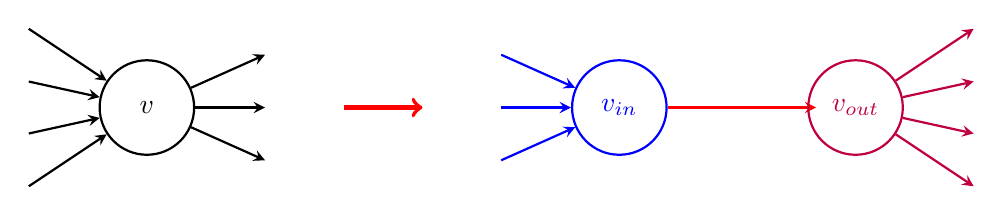
\begin{tikzpicture}

      % Define styles
      \tikzset{
          voltage node/.style={
              draw,
              circle,
              minimum size=1.2cm,
              thick
          },
          arrow style/.style={
              ->,
              >=stealth,
              thick
          }
      }

      % Left figure
      % Node v with 4 in-edges and 3 out-edges
      \node[voltage node] (v1) at (0,0) {$v$};

      % In-edges
      \draw[arrow style] (-1.5, 1) -- (v1);
      \draw[arrow style] (-1.5, 0.33) -- (v1);
      \draw[arrow style] (-1.5, -0.33) -- (v1);
      \draw[arrow style] (-1.5, -1) -- (v1);

      % Out-edges
      \draw[arrow style] (v1) -- (1.5, 0.67);
      \draw[arrow style] (v1) -- (1.5, 0);
      \draw[arrow style] (v1) -- (1.5, -0.67);

      % Arrow between figures
      \draw[->, line width=1.5pt, red] (2.5,0) -- (3.5,0);

      % Right figure
      % Node v_in with 3 in-edges
      \node[voltage node, blue] (v2) at (6,0) {$v_{in}$};
      \draw[arrow style, blue] (4.5, 0.67) -- (v2);
      \draw[arrow style, blue] (4.5, 0) -- (v2);
      \draw[arrow style, blue] (4.5, -0.67) -- (v2);

      % Connection between v_in and v_out
      \draw[arrow style, red] (v2) -- (8.5,0);

      % Node v_out with 4 out-edges
      \node[voltage node, purple] (v3) at (9,0) {$v_{out}$};
      \draw[arrow style, purple] (v3) -- (10.5, 1);
      \draw[arrow style, purple] (v3) -- (10.5, 0.33);
      \draw[arrow style, purple] (v3) -- (10.5, -0.33);
      \draw[arrow style, purple] (v3) -- (10.5, -1);

      \end{tikzpicture}
      \caption{} 
      \label{fig:undirected_ex}
    \end{figure}
  \end{example}

  \begin{example}[Maximum Bipartite Matching]
    Another application is in \textbf{bipartite matching}, which for an undirected bipartite graph $G(V, E)$ with $V = A \sqcup B$, is a subset of the edges $M \subset E$ s.t. no 2 edges in $M$ share an endpoint. The goal is to find the maximum bipartite matching, i.e. the matching with the greatest total weight. 

    \begin{figure}[H]
      \centering 
      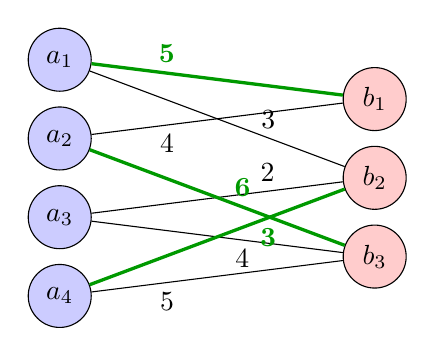
\begin{tikzpicture}[
          blue node/.style={draw, circle, fill=blue!20, minimum size=0.8cm},
          red node/.style={draw, circle, fill=red!20, minimum size=0.8cm},
          normal edge/.style={thin, black},
          matching edge/.style={very thick, green!60!black},
          normal weight/.style={black},
          matching weight/.style={green!60!black, font=\bfseries}
      ]

      % Left (blue) nodes
      \node[blue node] (a1) at (0,3) {$a_1$};
      \node[blue node] (a2) at (0,2) {$a_2$};
      \node[blue node] (a3) at (0,1) {$a_3$};
      \node[blue node] (a4) at (0,0) {$a_4$};

      % Right (red) nodes
      \node[red node] (b1) at (4,2.5) {$b_1$};
      \node[red node] (b2) at (4,1.5) {$b_2$};
      \node[red node] (b3) at (4,0.5) {$b_3$};

      % Regular edges with weights
      \draw[normal edge] (a1) -- node[above, pos=0.7] {3} (b2);
      \draw[normal edge] (a2) -- node[below, pos=0.3] {4} (b1);
      \draw[normal edge] (a3) -- node[above, pos=0.7] {2} (b2);
      \draw[normal edge] (a3) -- node[below, pos=0.6] {4} (b3);
      \draw[normal edge] (a4) -- node[below, pos=0.3] {5} (b3);

      % Maximum matching edges (highlighted in green)
      \draw[matching edge] (a1) -- node[above, pos=0.3, matching weight] {5} (b1);
      \draw[matching edge] (a2) -- node[above, pos=0.6, matching weight] {6} (b3);
      \draw[matching edge] (a4) -- node[below, pos=0.7, matching weight] {3} (b2);

      \end{tikzpicture}
      \caption{A bipartite matching} 
      \label{fig:bipartite_matching}
    \end{figure}

    The general idea is to take an undirected graph, convert it to a flow network, compute the max flow, i.e. min cut, and then translate it back into the undirected graph solution.  
    \begin{enumerate}
      \item Construct the flow network $G^\prime = (V^\prime, E^\prime)$, where $V^\prime = V \cup \{s, t\}$, with additional edges going from $s$ to $A$ and $B$ to $t$ all with weights $1$. Replace the middle edges with directed edges towards the flow with the same weight (though it can be any weight at least 1). 

      \begin{figure}[H]
        \centering 
        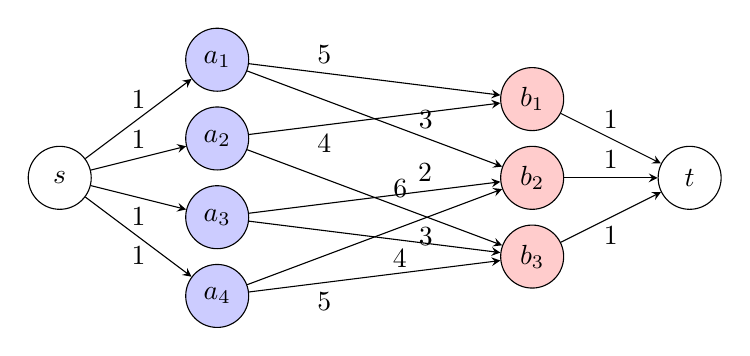
\begin{tikzpicture}[
            blue node/.style={draw, circle, fill=blue!20, minimum size=0.8cm},
            red node/.style={draw, circle, fill=red!20, minimum size=0.8cm},
            special node/.style={draw, circle, minimum size=0.8cm},
            edge/.style={->, >=stealth}
        ]

        % Source and sink nodes
        \node[special node] (s) at (-2,1.5) {$s$};
        \node[special node] (t) at (6,1.5) {$t$};

        % Left (blue) nodes
        \node[blue node] (a1) at (0,3) {$a_1$};
        \node[blue node] (a2) at (0,2) {$a_2$};
        \node[blue node] (a3) at (0,1) {$a_3$};
        \node[blue node] (a4) at (0,0) {$a_4$};

        % Right (red) nodes
        \node[red node] (b1) at (4,2.5) {$b_1$};
        \node[red node] (b2) at (4,1.5) {$b_2$};
        \node[red node] (b3) at (4,0.5) {$b_3$};

        % Edges from source to A nodes with weight 1
        \draw[edge] (s) -- node[above] {1} (a1);
        \draw[edge] (s) -- node[above] {1} (a2);
        \draw[edge] (s) -- node[below] {1} (a3);
        \draw[edge] (s) -- node[below] {1} (a4);

        % Edges from B nodes to sink with weight 1
        \draw[edge] (b1) -- node[above] {1} (t);
        \draw[edge] (b2) -- node[above] {1} (t);
        \draw[edge] (b3) -- node[below] {1} (t);

        % Middle edges (directed A to B) with original weights
        \draw[edge] (a1) -- node[above, pos=0.3] {5} (b1);
        \draw[edge] (a1) -- node[above, pos=0.7] {3} (b2);
        \draw[edge] (a2) -- node[below, pos=0.3] {4} (b1);
        \draw[edge] (a2) -- node[above, pos=0.6] {6} (b3);
        \draw[edge] (a3) -- node[above, pos=0.7] {2} (b2);
        \draw[edge] (a3) -- node[below, pos=0.6] {4} (b3);
        \draw[edge] (a4) -- node[below, pos=0.7] {3} (b2);
        \draw[edge] (a4) -- node[below, pos=0.3] {5} (b3);

        \end{tikzpicture}

        \label{fig:g_prime}
      \end{figure}

      \item Compute max flow $f$ in $G^\prime$. 
      \item Return $M = \{ (u \rightarrow v) \in E \mid f(u \rightarrow v) = 1 \}$. This can be done using the flow decomposition or just by looking at the edges in our flow with value $1$ and mapping it to the corresponding undirected bipartite graph. 
    \end{enumerate}
    To see correctness, we claim that there exists a matching $M$ in $G$ of size $k$ iff there exists a flow $f$ in $G^\prime$ with $|f|= k$, and therefore the max matching corresponds to the max flow. Constructing the flow network is $O(N + M)$ since $N^\prime = N + 2$ and $M^\prime = M + N$. Computing the max-flow is $O(N^\prime M^\prime)$ or $O(M^\prime |f|)$ depending on if we use Orlin's or Ford-Fulkerson, but either one is $O(NM)$. Then mapping it back to $M$ might take $O(M)$, so the total time is $O(NM)$. 
  \end{example}

